\title{CFD laboratory 4\\Flow around a circular cylinder in the sub-critical regime}
\author{
        Sergio M. Vanegas A.\\
        Francesco de Pas\\
                Department of Mathematics\\
        Polimi---Politecnico di Milano\\
        Milano, Italia
}
\date{\today}

\documentclass[12pt]{article}

\usepackage{amsmath}
\usepackage{graphicx}
\usepackage{siunitx}

\begin{document}
\maketitle

\begin{abstract} 
        The fourth test case is the flow around a circular cylinder in the sub-critical regime. The cylinder is considered with infinite height to avoid side effects. The flow develops from the free-stream profile $U_\infty$ in the form of a laminar boundary layer that, after separation at about 82° from the leading edge, generates a turbulent wake with some periodic behavior. The phenomenon is inherently unsteady even at the macro-scale and therefore it requires solving the U-RANS, which might be computationally demanding even for a 2D problem. As a consequence it is here performed the grid independence study for a steady state (RANS) model, and then use the same grid settings for the subsequent U-RANS simulation.\cite{FL:06}
 
        \begin{figure}[!ht]
                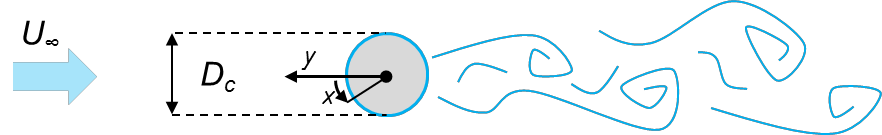
\includegraphics[width=\textwidth]{Flow_Sketch.png}
                \centering
                \caption{}
                \label{fig:flow_sketch}
        \end{figure}
 
 
\end{abstract}

\section{Introduction}

        In the sub-critical regime, the laminar boundary layer developing over the walls of the cylinder separates at about 82° from the front stagnation point, and a large, turbulent wake generates downstream. The pressure distribution over the walls of the cylinder, shown in Figure~\ref{fig:p_d}, agrees with the potential flow solution only in the front part of the body. The separation point is just at the beginning of the region of adverse pressure gradient, and it can be easily recognized in the figure since the wall pressure in the wake region is broadly uniform. Additionally, the wall shear stress is zero at the point of separation.


        \begin{figure}[!ht]
                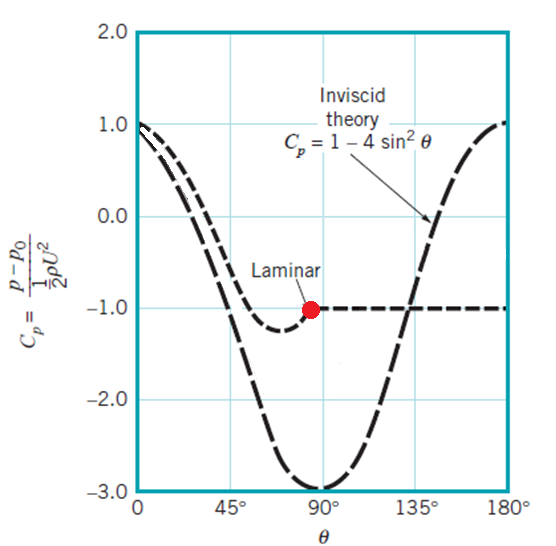
\includegraphics[width=\textwidth]{Pressure_Distribution.png}
                \centering
                \caption{}
                \label{fig:p_d}
        \end{figure}

        The drag coefficient of a circular cylinder with infinite length is defined as: $$C_D = \frac{\frac{F_D}{H}}{\frac{1}{2} \rho \left(\frac{A_D}{H}\right) U_\infty^2} = \frac{\frac{F_D}{H}}{\frac{1}{2} \rho \left(\frac{D_C H}{H}\right) U_\infty^2} = \frac{\frac{F_D}{H}}{\frac{1}{2} \rho D_C U_\infty^2}$$ and it is a function of $\text{Re}_D$ and the relative roughness $\frac{s}{D_C}$. In the sub-critical regime, $C_D$ is nearly constant with $\text{Re}_D$, and it is not much affected by the roughness. Such constant value is around 1.2, as is it evident from Figure~\ref{fig:dragtrend}.

        \begin{figure}[!ht]
                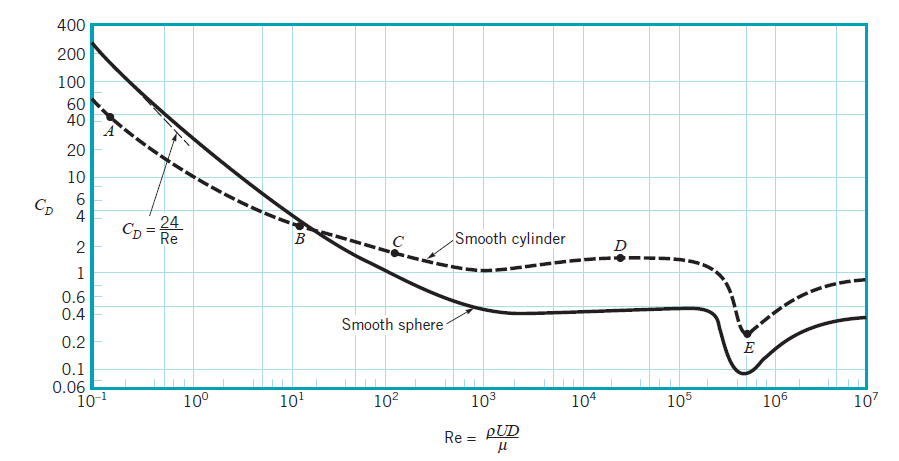
\includegraphics[width=\textwidth]{DragCoefficient_Trend.png}
                \centering
                \caption{}
                \label{fig:dragtrend}
        \end{figure}

        Finally, the dimensionless Strouhal number quantifies the characteristic frequency of the turbulent wake, \textit{f},and it is defined as $St = \frac{f*D_C}{U_\infty}$. The paper by Fey et al. (1998) provides a correlation to estimate \textit{St} as a function of $\text{Re}_D$, according to which, in the sub-critical regime, \textit{St} varies between 0.185 and 0.21 Figure~\ref{fig:strouhal}.


 \begin{figure}[!ht]
                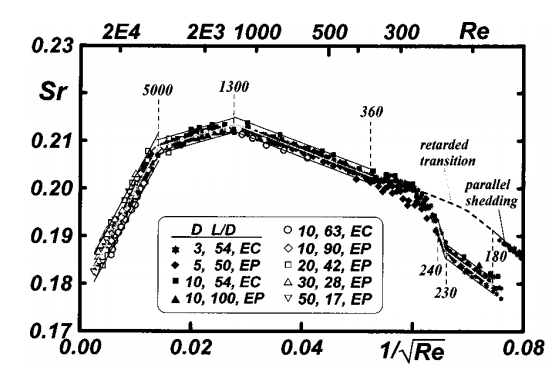
\includegraphics[width=\textwidth]{Strouhal.png}
                \centering
                \caption{}
                \label{fig:strouhal}
        \end{figure}


        The configuration of the problem is as follows:
        \begin{itemize}
                \item Diameter \( D_c = 0.06 \: m \),
                \item Free-stream velocity \( U_\infty = 0.4 \: m/s \),
                \item Bulk velocity \( U_b = 5 \: mm/s \),
                \item Fluid: Water at \( 20^{\circ}C \; \rho = 998.23 \: kg/m^3\;( \mu=1.006*10^{-6} \:m^2/s\)).
        \end{itemize}


        \paragraph{Outline}
        The remainder of the report is organized as follows: Section~\ref{sec:Steady-state precursor} provides some suitable results concerning the Grid Independence Study performed on RANS solutions; Section~\ref{sec:URAN} instead makes use of URANS in order to focus on the temporal evolution  of the process; Section~\ref{sec:Comparison with Literature} compares the results obtained with literature ones and finally  Section~\ref{sec:Comparison RANS vs URANS} compares RANS and URANS solutions, taking into account the inviscid flow potential solutions.
      
\section{Steady-state precursor} \label{sec:Steady-state precursor}

        The following Grid-Independence study is applied on RANS solution.   Despite in principle RANS solutions do not provide a trustful representation of the physical phenomenon under investigation, this choice can been consider a practical compromise to face the heavy URANS  computational cost. The variables under investigation are:  the distributions of wall pressure and wall shear stress, the drag coefficient and the position of the separation point, inferred from the wall pressure and the wall shear stresses.In particular the separation point was inferred by the wall pressure approximating the wall pressure second derivative (through finite differences of order 8) and looking for its inflection point. The separation point was instead inferred by the shear stress imposing it as the shear stress zero.
        
        The study was performed by setting \textit{3} different meshes along the $\Theta$ coordinate: 120, 180 and 360 equally spaced cells, while mantaining the $\rho$ grid fixed to 100 cells distributed through a Geometric law with a coefficient of...

        Figure~\ref{fig:drag_independence}, Figure~\ref{fig:pression_ind}, and Figure~\ref{fig:wall_ind} show our results.

        \begin{figure}[!ht]
                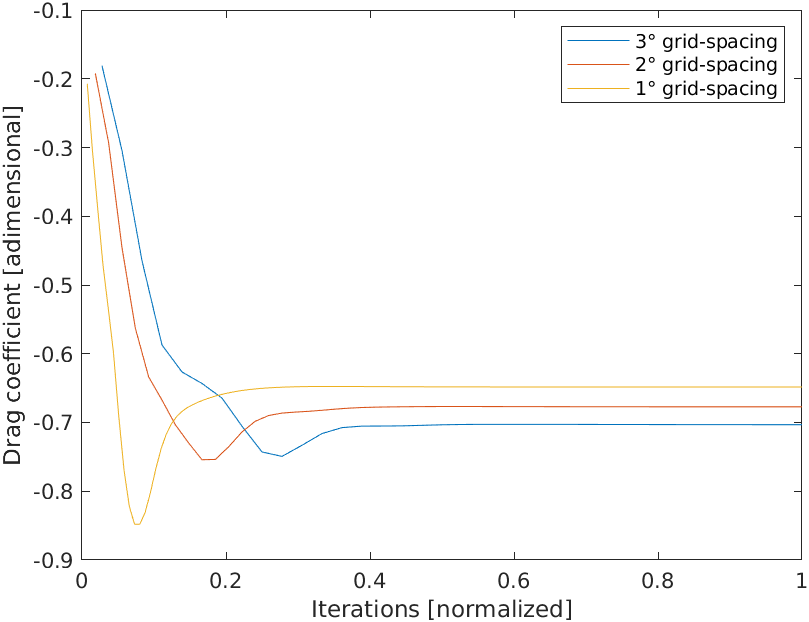
\includegraphics[width=\textwidth]{DragCoefficient_Independence.png}
                \centering
                \caption{}
                \label{fig:drag_independence}
        \end{figure}

        \begin{figure}[!ht]
                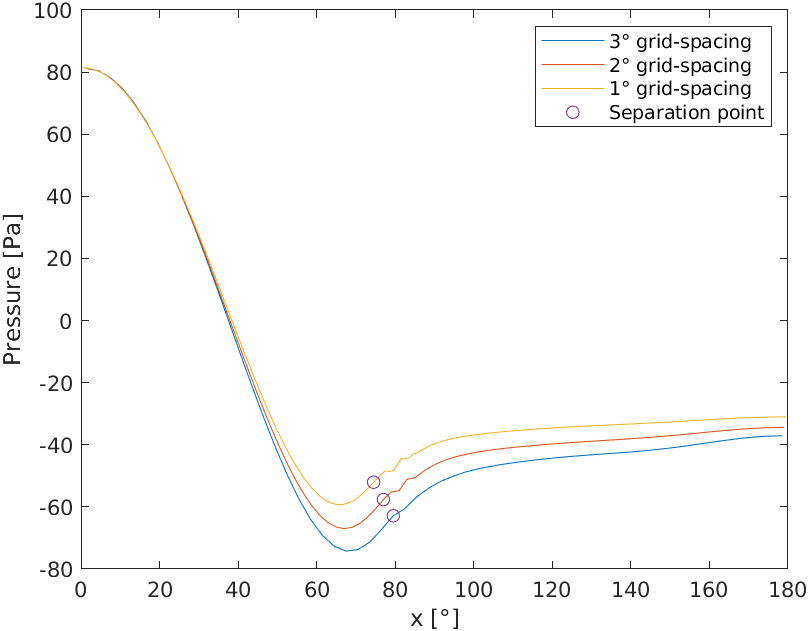
\includegraphics[width=\textwidth]{Pressure_Independence.png}
                \centering
                \caption{}
                \label{fig:pression_ind}
        \end{figure}

        \begin{figure}[!ht]
                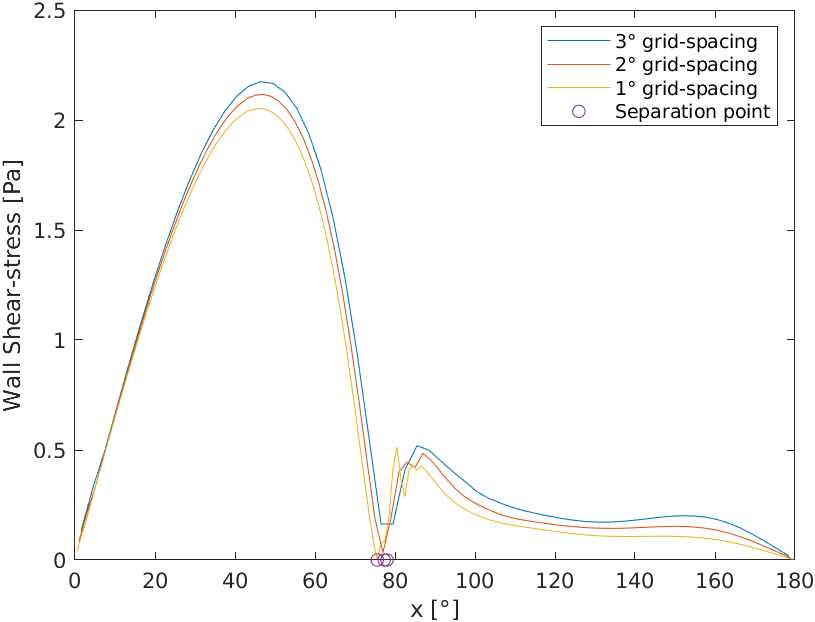
\includegraphics[width=\textwidth]{WallShearStress_Independence.png}
                \centering
                \caption{X-velocity Y-profile per delta-step}
                \label{fig:wall_ind}
        \end{figure}


        According to experimental results separation point s should lie at $$ 82 ^\circ $$, and our plot quite respects this result.

\section{Unsteady-state modelling} \label{sec:URAN}
        In this section we'll make use of our results from URANS simulations. To launch these simulations we re-started from the converged steady-state solutions exploiting the finer grid setting.

        We defined as suitable total simulation time to observe periodicity in the macroscopic flow: 60 s. Then, we performed a sensibility analysis with respect to the time-step of time discretization; we considered three different timesteps, ensuring their value to be much smaller with respect to the total time-scal and bigger than microscopic turbolent time-scales. These were:

        \begin{itemize}
                \item $0.06 s$ ($0.1\%$ of the total simulation time).
                \item $0.10 s$ ($0.17\%$ of the total simulation time).
                \item $0.20 s$ ($0.33\%$ of the total simulation time).
        \end{itemize}
        
        At each time-step we considered as target parameter: forces on the \textit{X} and \textit{Y} axis.

        The behaviour of the Drag and Lift force with the 3 different values imposed can be seen respectively in Figure~\ref{fig:drag} and Figure~\ref{fig:lift}. This figures appear to well describe the phenomenon under investigation, nevertheless in the lift case, the coarser time-step seems not to perfectly catch the frequency of lift force oscillations, probably due to the bigger window of the moving average operator.

        Finally both their trend stabilize since from 45\:s, showing that the total simulation time chosen is correct.

        \begin{figure}[!ht]
                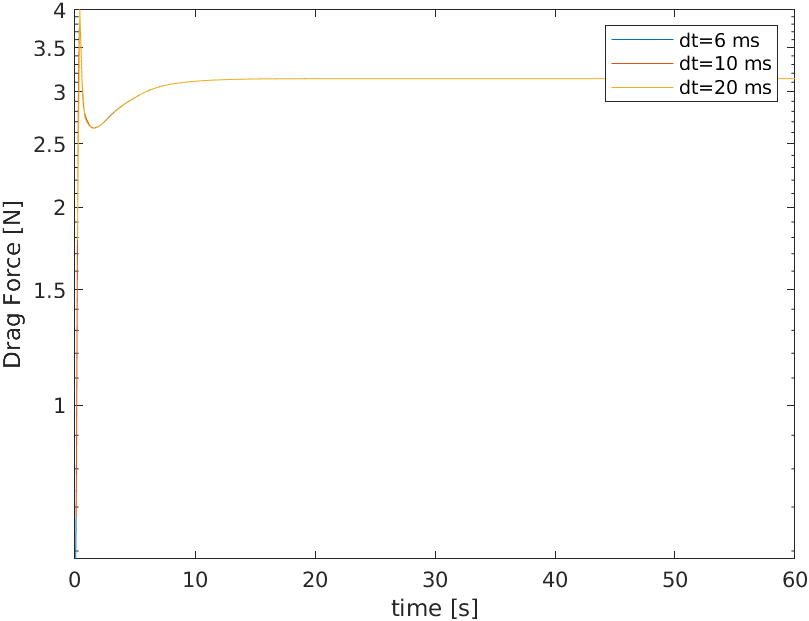
\includegraphics[width=\textwidth]{DragForce.png}
                \centering
                \caption{}
                \label{fig:drag}
        \end{figure}

        \begin{figure}[!ht]
                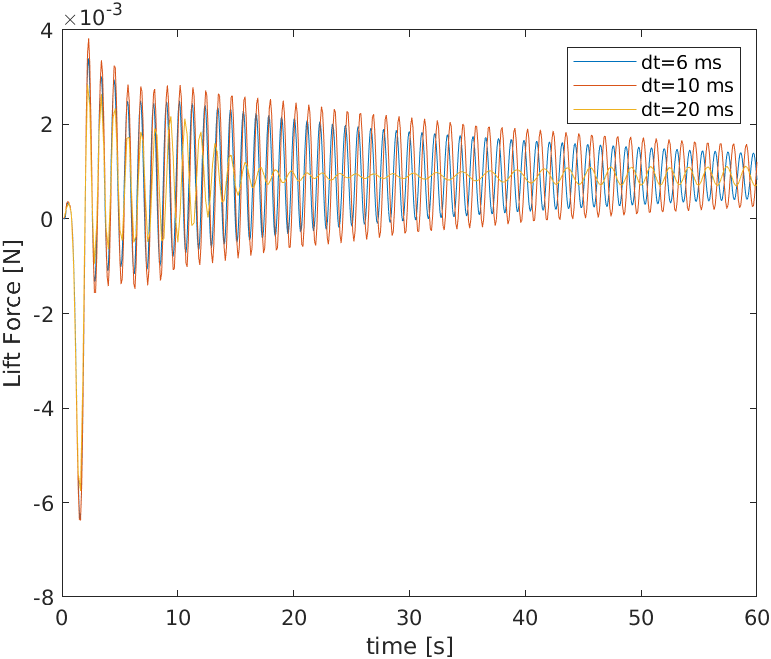
\includegraphics[width=\textwidth]{LiftForce.png}
                \centering
                \caption{}
                \label{fig:lift}
        \end{figure}

        Regarding the Drag and Lift coefficients evolution over time, we used the $0.06 s$ timestep; the numerical results are shown in Figure~\ref{fig:drag_coeff} and  Figure~\ref{fig:lift_coeff}. At first glance they seem consistent with the phisical phenomenon, since the lift coefficient oscillations are 0-averaged, while drag coefficients oscillations are positively averaged. 

        \begin{figure}[!ht]
                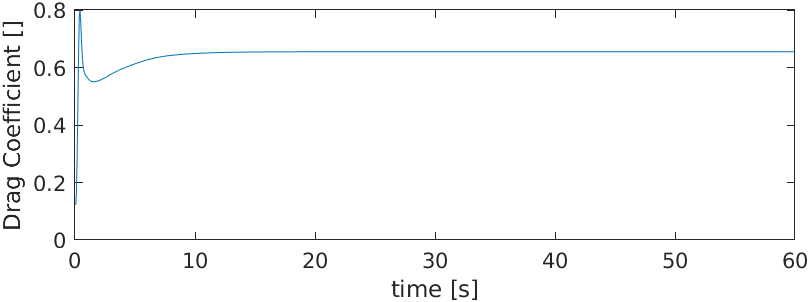
\includegraphics[width=\textwidth]{Drag_Coefficient.png}
                \centering
                \caption{}
                \label{fig:drag_coeff}
        \end{figure}
                \begin{figure}[!ht]
                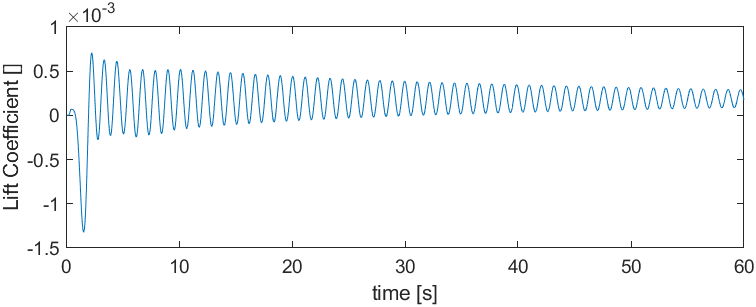
\includegraphics[width=\textwidth]{Lift_Coefficient.png}
                \centering
                \caption{}
                \label{fig:lift_coeff}
        \end{figure}


        in order to compare the coefficients, we made used of the plots of Figure(). As it can be clearly seen the both the amplitude of the drag coefficient oscillations is of the order of $\num{1E-6}$, while its frequency is nearly $10$, while for the lift one, consistently with the phisical phenomenon the amplitude is $\num{1E3}$ times bigger, being of the order of $\num{2E-3}$, while its frequency smaller, it is of order $1$. 

        The averaged Drag Coefficients is $\num{0.6468}$, while the averaged Lift Coefficient is $\num{1.89E-4}$. The computed numerical value does not match well the reference one of Figure~\ref{fig:dragtrend}, that suggests $1.5$.

        For the Strouhal number, its computed value was $0.1365$, (slightly below the expectations of Figure~\ref{fig:strouhal}, but well within the numerical error range). 

\bibliographystyle{abbrv}
\bibliography{main}

\end{document}
